\documentclass[a4paper, 11pt]{article}
\usepackage[french]{babel}
\usepackage[utf8]{inputenc}
\usepackage[T1]{fontenc}
\usepackage{datetime}
\usepackage{float}
\usepackage{eurosym}
\usepackage{comment} % enables the use of multi-line comments (\ifx \fi)
\usepackage{graphicx}

\usepackage{fullpage} % changes the margin
\begin{document}
%Header-Make sure you update this information!!!!
\noindent
\large\textbf{Cahier des charges} \hfill \textbf{Distribution de l'eau en Haïti} \\
\normalsize Deknop Céline \hfill Université catholique de Louvain \\
Hallet Adrien \hfill \today \\
Strebelle Sébastien

\section*{Abstract}
Cahier des charges du projet de gestion de distribution d'eau en Haïti, mémoire UCLouvain 2018-2019. Destiné aux intervenants du projet et contenant les propositions pour la future application.
\hrule
\section{Glossaire}
% Liste exhaustive de tous les termes pouvant prêter à confusion
  \begin{description} %ToDo : trouver un moyen de display ça beau, je sais pas si c'est l'idéal. Aussi y'a pas moyen d'auto-sort par ordre alphabétique ?
    %ToDo 2 : définir les termes
    %ToDo 3 : ordonner alphabétiquement le truc si on peut pas le faire automatiquement
    %ToDo 4 : check le document résuglièrement et ajouter tous les termes qui peuvent prêter à confusion
    \item[CAEPA]
    \item[DINEPA]
    \item[HTG]
    \item[Utilisateur]
    \item[Application]
    \item[Permission]
    \item[Réseau]
    \item[Fontaine]
    \item[Kiosque]
    \item[Réservoir]
    \item[Prise individuelle]
  \end{description}
\section{Introduction}
% Contexte de l'application
\section{Types d'utilisateurs}
  \begin{description}
    \item[Gestionnaire de zone] est un utilisateur qui gère un groupe de gestionnaires de fontaines. Il dispose des mêmes permissions que les gestionnaires de fontaines dans sa zone et peut donc agir comme un gestionnaire de fontaine. En plus, le gestionnaire de zone peut créer des gestionnaires de fontaines et des techniciens/plombiers et leur assigner des permissions sur les éléments du réseau.

    \emph{Exemple 1 : Protos ou la DINEPA peuvent être assignés en tant que gestionnaires de zone ayant les accès sur tous les systèmes et agir en tant que gestionnaires généraux de tout le système. Ils peuvent donc consulter toutes les informations rapportées par les autres utilisateurs.}

    \emph{Exemple 2 : un CAEPA pourrait être assigné en tant que gestionnaire de zone et avoir accès aux infrastructures du réseau de distribution dans sa zone géographique et ainsi consulter les informations et les modifier pour venir en aide aux gestionnaires de fontaine.}

    \item[Gestionnaire de fontaines] est un utilisateur auquel on assigne un ou plusieurs éléments du réseau de distribution de type "sortie" (fontaine, kiosque, réservoir, branchement individuel) dont il est responsable.
    Il est responsable de la gestion des utilisateurs dans sa zone et les ajoute/supprime dans le système lorsque c'est nécessaire (naissance, décès, déménagement).
    Il utilise l'application pour signaler des problèmes et ainsi pouvoir avertir le technicien/plombier et sa hiérarchie. Chaque mois, le gestionnaire de fontaines utilise l'application pour déposer un rapport. Ce rapport contient, pour chaque élément sous la responsabilité du gestionnaire de fontaines, les quantités d'eau distribuées, les recettes (HTG), l'état (en service, hors service). Une section générale (une seule fois par rapport) déclare également les heures et jours de service du gestionnaire de fontaines.

    \emph{Exemple : une personne chargée de gérer un point d'eau pourrait être un gestionnaire de fontaine. Il peut ainsi utiliser l'application pour envoyer mensuellement les données, ajouter les utilisateurs lorsque nécessaire et déclarer les problèmes.}

    \item[Technicien/Plombier] est un utilisateur auquel on assigne des éléments du réseau de distribution (fontaine, réservoir, prise individuelle, etc). Chaque technicien/plombier utilise l'application pour voir les problèmes déclarés par les gestionnaires de fontaines. Il peut utiliser l'application pour répondre aux demandes d'intervention pour demander plus d'informations ou proposer une solution si le déplacement n'est pas nécessaire. Il peut modifier l'état d'un probème et le marquer en cours de résolution ou résolu une fois l'intervention terminée.

    \emph{Exemple : un technicien plombier démarrant sa journée peut consulter l'application et voir quels sont les problèmes qui requièrent son attention. Il peut dialoguer avec les gestionnaires et modifier l'état des problèmes afin qu'à terme le réseau fonctionne sans problème.}
  \end{description}
  \subsection{Questions}
  % Questions
  % Cas pratique de la sécurité de l'administrateur
\section{Fonctionnalités}
% Liste exhaustive des fonctionnalités de l'application
  \subsection{Questions}
\section{Exemples principaux}
  \subsection{Fonctionnement général}
    \begin{figure}[H]
        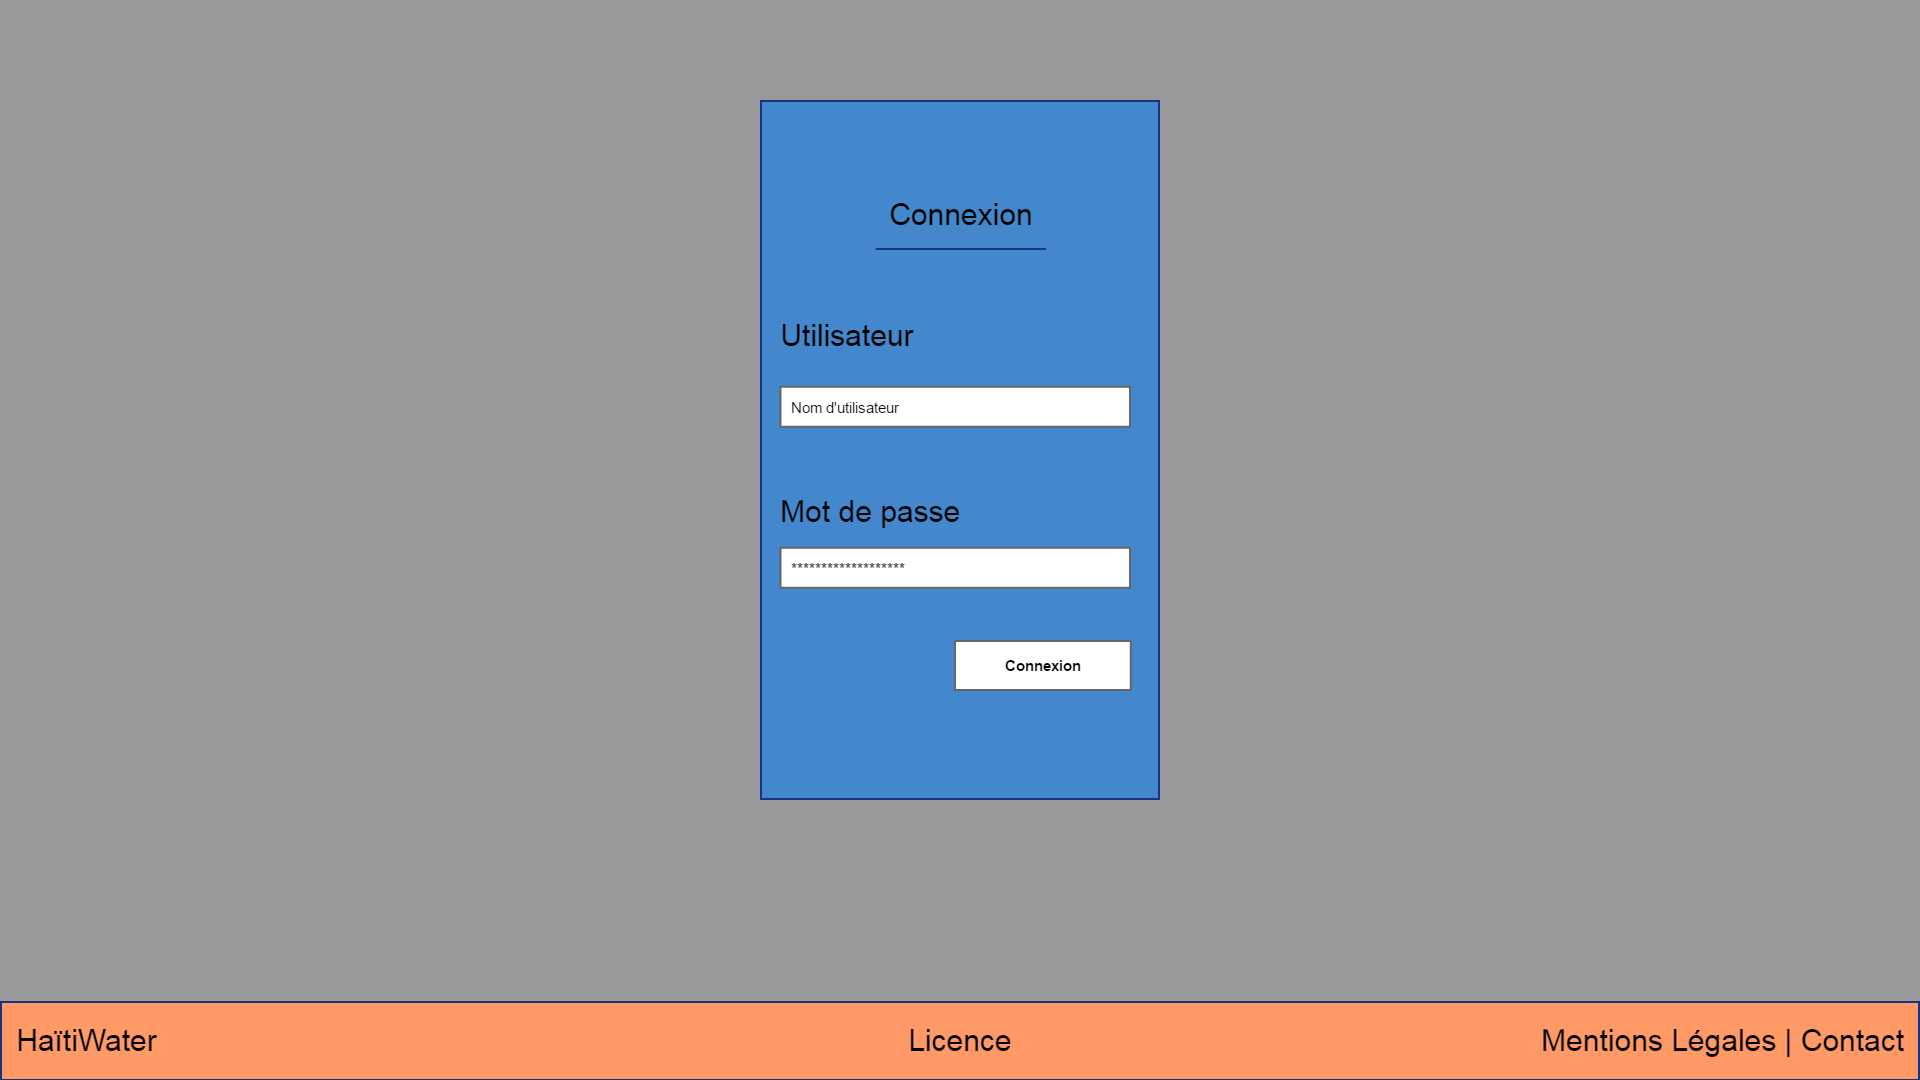
\includegraphics[width=\textwidth]{Cahier_des_Charges/login}
        \caption{\'Ecran d'identification}
        \label{fig:login}
    \end{figure}

    L'application fonctionne sur base des permissions de chaque utilisateur. La figure~\ref{fig:login} montre l'écran sur lequel tout utilisateur de l'application commence afin de pouvoir se connecter. Chaque utilisateur dispose au préalable de ses identifiants de connexion qui lui ont été fournis par sa hiérarchie.

    \begin{figure}[H]
        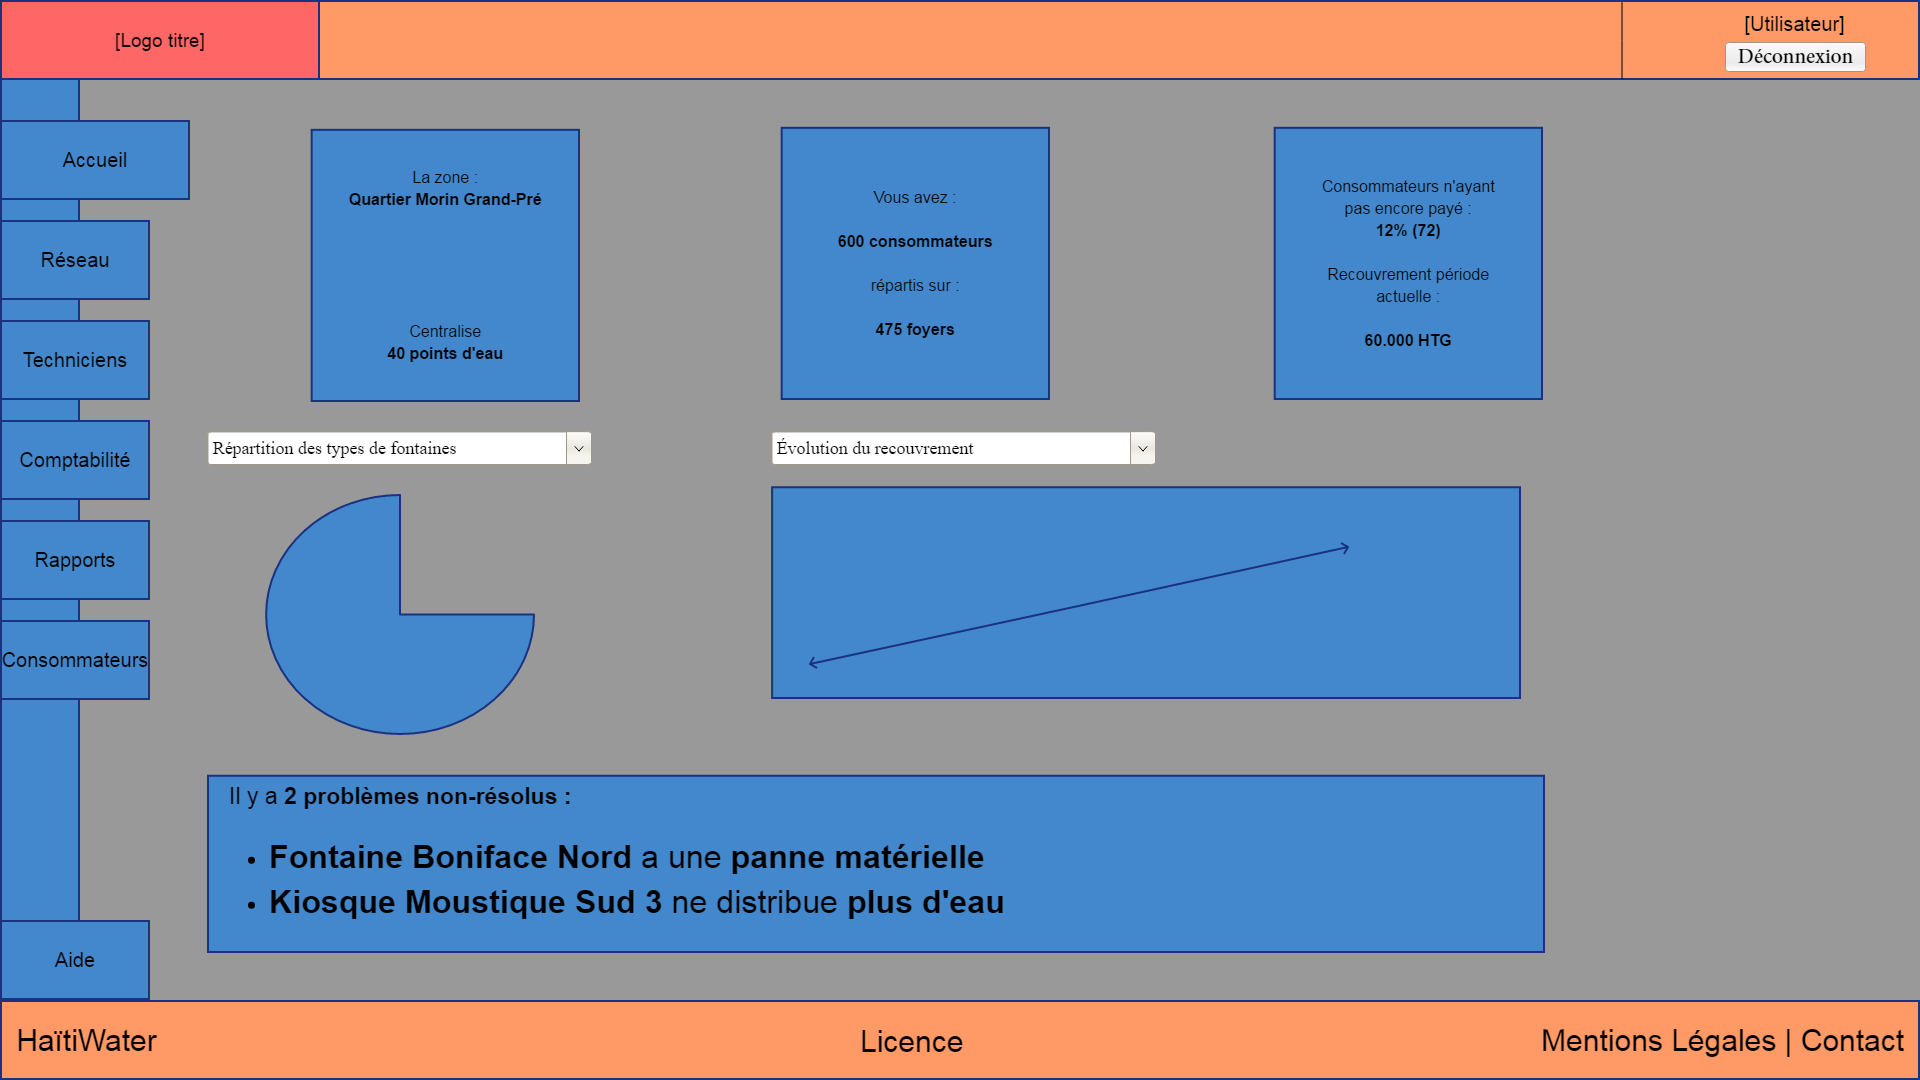
\includegraphics[width=\textwidth]{Cahier_des_Charges/accueil} % ToDo : modifier l'écran pour montrer un exemple
        \caption{\'Ecran d'accueil}
        \label{fig:dashboard}
    \end{figure}

    Une fois connecté, l'utilisateur dispose d'un écran d'accueil (figure~\ref{fig:dashboard}) personnalisé qui affiche des informations en fonction de son rôle. Un technicien voit la liste et le nombre des interventions en attente.
    \begin{description}
      \item[Un gestionnaire de zone et gestionnaire de fontaines] voient les sorties d'eau du réseau dont ils sont responsables (fontaines, réservoirs et prises individuelles) et leur état de fonctionnement (en service, hors service, en cours de réparation). Ils disposent également de statistiques mises en avant (quantité d'eau distribuée, somme des recettes, nombre d'utilisateurs) afin de proposer un accès rapide aux informations les plus importantes.\\
      Le gestionnaire de zone dispose en plus de la liste des gestionnaires de fontaines sous sa responsabilité.
      \item[Un technicien/plombier] voit le nombre et la liste des interventions en attente.
    \end{description}
    Sur la gauche, chaque utilisateur voit le menu comprenant les pages auxquelles il a accès. Tous les utilisateurs n'ont pas les mêmes permissions. Le gestionnaire de zone peut voir tous les menus permettant de gérer le réseau, les consommateurs, les techniciens, les gestionnaires de fontaine et problèmes qui sont sous sa responsabilité. Le gestionnaire de fontaine peut voir le réseau auquel il est assigné, les consommateurs et problèmes des points sous sa responsabilité.


  \subsection{Gestionnaire de fontaine}
  \begin{figure}[H]
      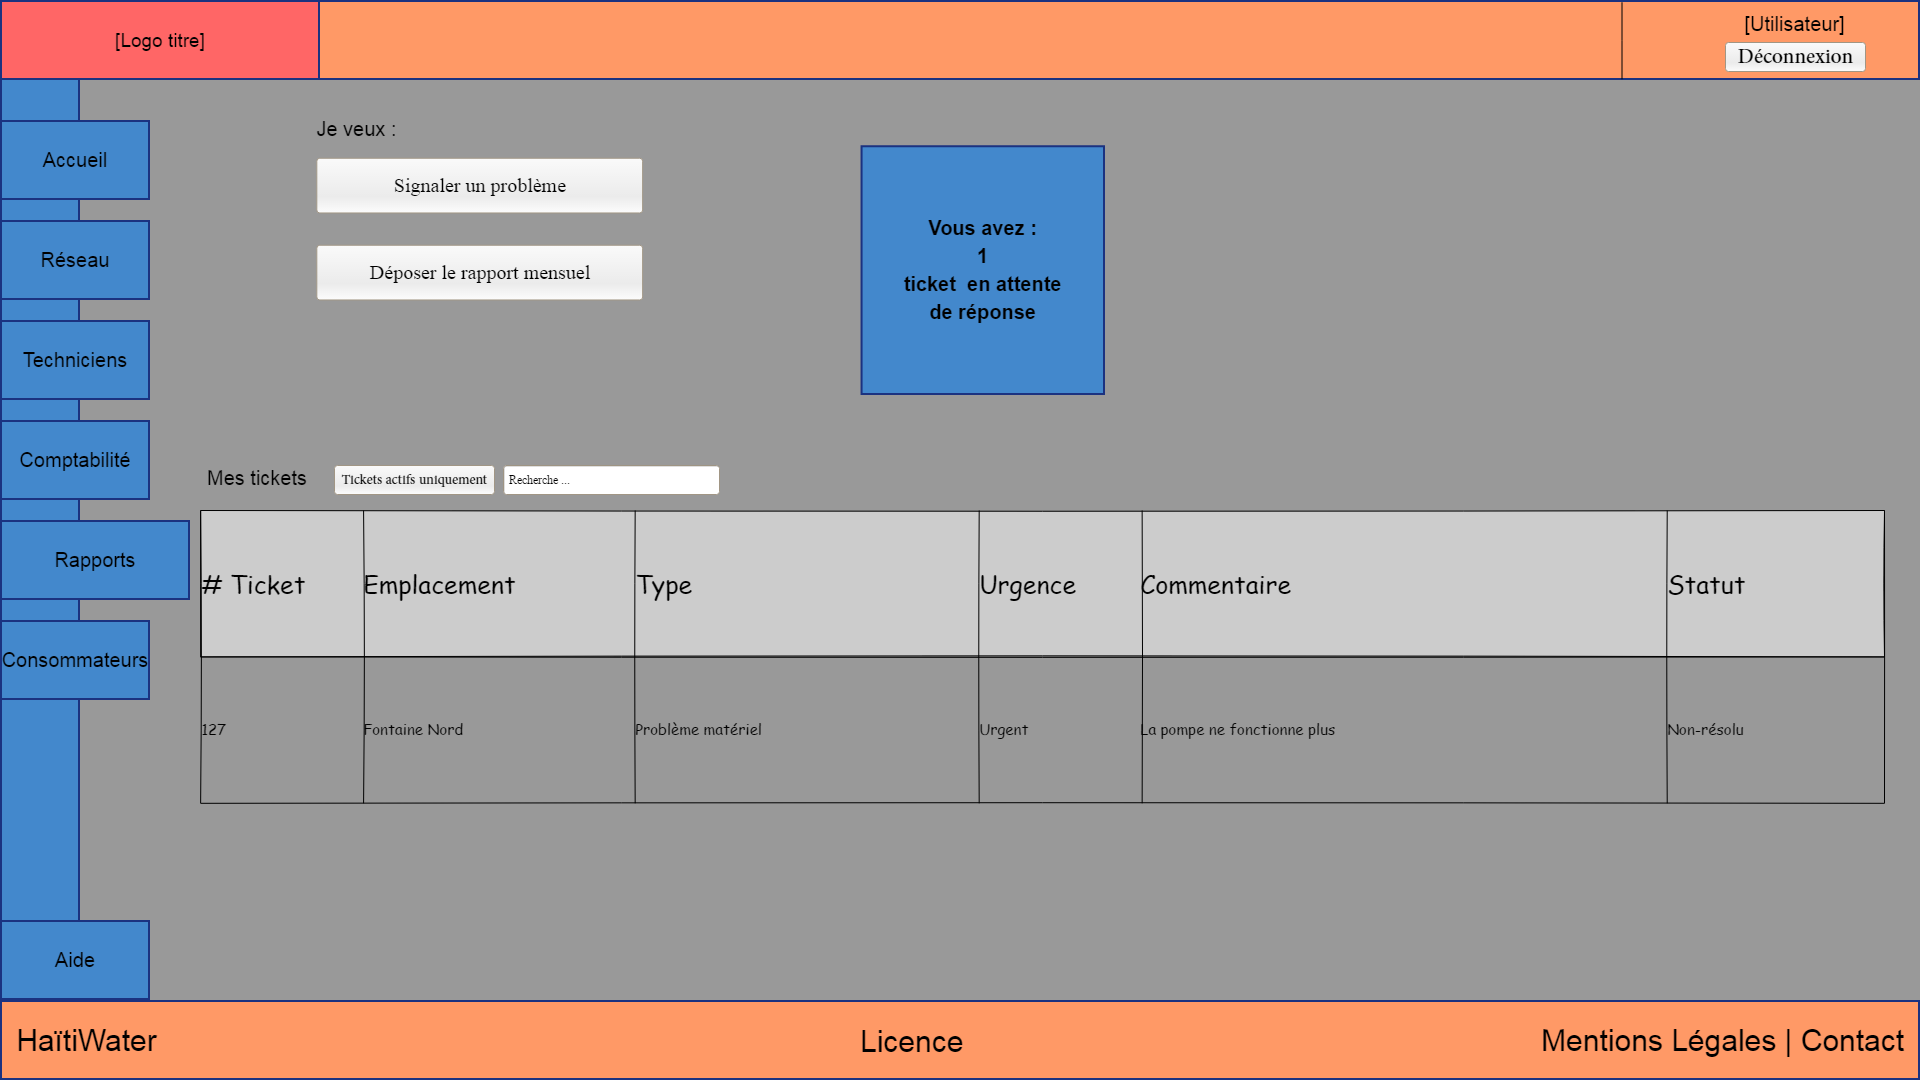
\includegraphics[width=\textwidth]{Cahier_des_Charges/rapports}
      \caption{Test}
      \label{fig:reports}
  \end{figure}

\section{Besoins non-fonctionnels}
% Explication des besoins non-fonctionnels
\section{Fonctionnement de la recherche de fonctionnalités}
% D'où viennent les idées
\section{Choix technolgiques}
% Point de vue purement "positif pour le projet" sans termes techniques
\end{document}
